\documentclass[prb,preprint]{revtex4-1} 
% The line above defines the type of LaTeX document.
% Note that AJP uses the same style as Phys. Rev. B (prb).

% The % character begins a comment, which continues to the end of the line.

\usepackage{amsmath}  % needed for \tfrac, \bmatrix, etc.
\usepackage{amsfonts} % needed for bold Greek, Fraktur, and blackboard bold
\usepackage{graphicx} % needed for figures
\usepackage{color}
\begin{document}

% Be sure to use the \title, \author, \affiliation, and \abstract macros
% to format your title page.  Don't use lower-level macros to  manually
% adjust the fonts and centering.

\title{Critical Temperature of YBCO and BSCCO Superconductors}
% In a long title you can use \\ to force a line break at a certain location.

\author{Ed Lipchus}
\affiliation{Hampshire College, Amherst, MA 01002}

% optional second address
% If there were a second author at the same address, we would put another 
% \author{} statement here.  Don't combine multiple authors in a single
% \author statement.


\author{Frances Yang}
\affiliation{Department of Physics, Smith College, Northampton, MA 01063}

% See the REVTeX documentation for more examples of author and affiliation lists.

\date{\today}

\begin{abstract}

Superconductors are materials that lose their electrical resistance when they fall below a certain temperature, called the critical temperature. We determined the critical temperatures for $\text{Yt}\text{Ba}_{2}\text{Cu}_{3}\text{O}_{7-\delta}$ to be $98.35\textrm{ K} \pm 7\textrm{ K}$. We found a single phase transition at $110\text{ K}\pm 9 \text{ K}$ for $\text{Bi}_{2}\text{Sr}_{2}\text{Ca}_{n-1}\text{Cu}_{n}\text{O}_{2n+4}$ as well.
The critical temperatures are found by passing a fixed current through a superconducting sample and measuring the change in voltage across the sample to determine its resistance. We describe the critical temperature as the temperature halfway through the transition from non-zero resistance to zero resistance. Previous measurement of the critical temperature for YBCO gives a critical temperature of 91 K. Our critical temperature for BSCCO is in agreement with previous measurements for $n=3$ phase found in the literature. This confirms that our BSCCO consists of mainly $n=3$, as indicated in the manual that came with our samples. We also saw agreement with a gneral decrease in critical temperature with an increase in current run through the YBCO sample, however the transition was uneven and distorted, so a specific difference in critical temperature could not be determined.


\end{abstract}
% AJP requires an abstract for all regular article submissions.
% Abstracts are optional for submissions to the "Notes and Discussions" section.

\maketitle % title page is now complete


\section{Introduction} % Section titles are automatically converted to all-caps.
% Section numbering is automatic.
In 1911, Kamerlingh Onnes discovered superconductivity in mercury.  
Instead of a gradual decrease in the electrical resistance as the temperature decreased, he found a sudden loss of resistance when the temperature went below 4.2 K. 
The temperature at which the resistance disappears is called the critical temperature.
In addition to having no resistance, superconductors also exhibit perfect diamagnetism, which means they exclude all magnetic field flux from their interior. 
This property, called the Meissner effect, was discovered in 1933.\cite{intro}
A common demonstration of the Meissner effect is to place a a magnet on top of a superconductor above its critical temperature. When the superconductor is cooled to become superconducting, the magnet will start to levitate above the superconductor. 

The main application of superconductors is in making high field magnets from superconducting wires. They can also be used to make levitation trains or to create magnetic fields used in magnetic resonance imaging and in high energy physics to accelerate and control the path of particles.\cite{kumar} 

Superconductivity has been found to occur in elements, alloys, binary compounds, and other materials.  
Roughly 70 years after superconductivity was discovered, ceramic materials with critical temperatures above the liquid nitrogen temperature of 77 K were found.\cite{melissinos} 
These ``high temperature'' superconductors were made up of alternating layers of rare earth atoms and copper and oxygen atoms.\cite{kumar} 
In our experiment, we look at two high temperature superconductors, $\text{Yt}\text{Ba}_{2}\text{Cu}_{3}\text{O}_{7-\delta}$ and $\text{Bi}_{2}\text{Sr}_{2}\text{Ca}_{n-1}\text{Cu}_{n}\text{O}_{2n+4}$, where $n=1,2,\text{ or },3$. %n=3 mainly for colorado superconductor 110 Tc
The amount of oxygen in $\text{Yt}\text{Ba}_{2}\text{Cu}_{3}\text{O}_{7-\delta}$ determines if the material will be superconducting.\cite{colo} The critical temperature of $\text{Yt}\text{Ba}_{2}\text{Cu}_{3}\text{O}_{7-\delta}$ is roughly 93 K.\cite{ybcotemp}
For $\text{Bi}_{2}\text{Sr}_{2}\text{Ca}_{n-1}\text{Cu}_{n}\text{O}_{2n+4}$, the critical temperature depends on the value of n.  
They are 20 K, 85 K, and 110 K, for $n=1,2,\text{ and }3$, respectively.\cite{temps}

\section{Procedure}
The YBCO and BSCCO superconductors were obtained from Colorado Superconductor Inc. The manual from Colorado Superconductor Inc. notes that the BSCCO samples consists of mainly $n=3$. Each superconductor  is contained in a brass casing with three pairs of leads. 
One pair was for attaching to the current source, another pair was used to measure voltage across the superconductor, and the last pair that of the thermocouple inside the casing. 
The thermocouple produces a voltage when one part of the circuit has a temperature different from a reference point.
We used different methods to measure the critical temperature of the two superconductors. 
For the YBCO, we connected it to a source with an alternating current of $\pm$1 mA. The alternating current provides a more accurate reading of the voltage across the sample, because it removes any offset the voltmeter may have.
The voltage across the YBCO sample, $V_{\text{YBCO}}$, and the voltage across the thermocouple junction, $V_{T}$ were measured with two nanovoltmeters. 
The voltage across the YBCO sample was converted into a resistance reading by the nanovoltmeter.
 \textcolor{blue}{Include circuit diagrams.} 

\textcolor{red}{Finally, didn't you do some measurements at other values of current? for example, 10 mA and 100 mA, in addition to 1 mA? YOu were supposed to, and I thought you had. I can't find those results anywhere in your paper. } 

We placed the superconductor inside a styrofoam cup filled with sand. 
The sand reduces the rate at which the superconductor heats up, which allows us to gather more data points. 
We cooled the YBCO sample by pouring liquid nitrogen into the styrofoam cup. We waited for the superconductor to settle to a minimum temperature. Then we recorded $V_{\text{YBCO}}$ and $V_{T}$ as it warmed up to above its critical temperature. 

We used a two-phase lock-in amplifier for the BSCCO experiment. An AC circuit set up for the measurement of resistance is susceptible to contributions from capacitors and inductors. 
Although there are no explicit capacitors or inductors in our circuit, they are effectively present due to the electrical cables used and construction of the circuit. 
The lock-in amplifier allows us to extract the resistance of superconductor from the other contributions. Since changes in $V_{\text{BSCCO}}$ due to resistance are in phase with applied voltage and the contributions of capacitors and inductors are out of phase, our signal is just the in phase component.  
Since the resistance of the BSCCO at room temperature is on the order of m$\Omega$s, we can generate an AC current with an RMS amplitude of approximately $\pm$1 mA in the circuit by connecting the BSCCO in series with a 1 k$\Omega$ resistor, and with a AC voltage source with an RMS amplitude of 1 V. 



\section{Results and Analysis}

First, to convert our thermocouple voltage into a usable temperature, we transcribed the chart provided in the Colorado Superconductor Inc. experiment manual that came with the YBCO and BSCCO samples and and plotted temperature vs voltage (see Fig. \ref{TCplot}). While it was best fit piecemeal, a single curve was able to cover our temperature range, and we used that function to convert our thermocouple voltages in later fits.

\begin{figure}[h!]
\centering
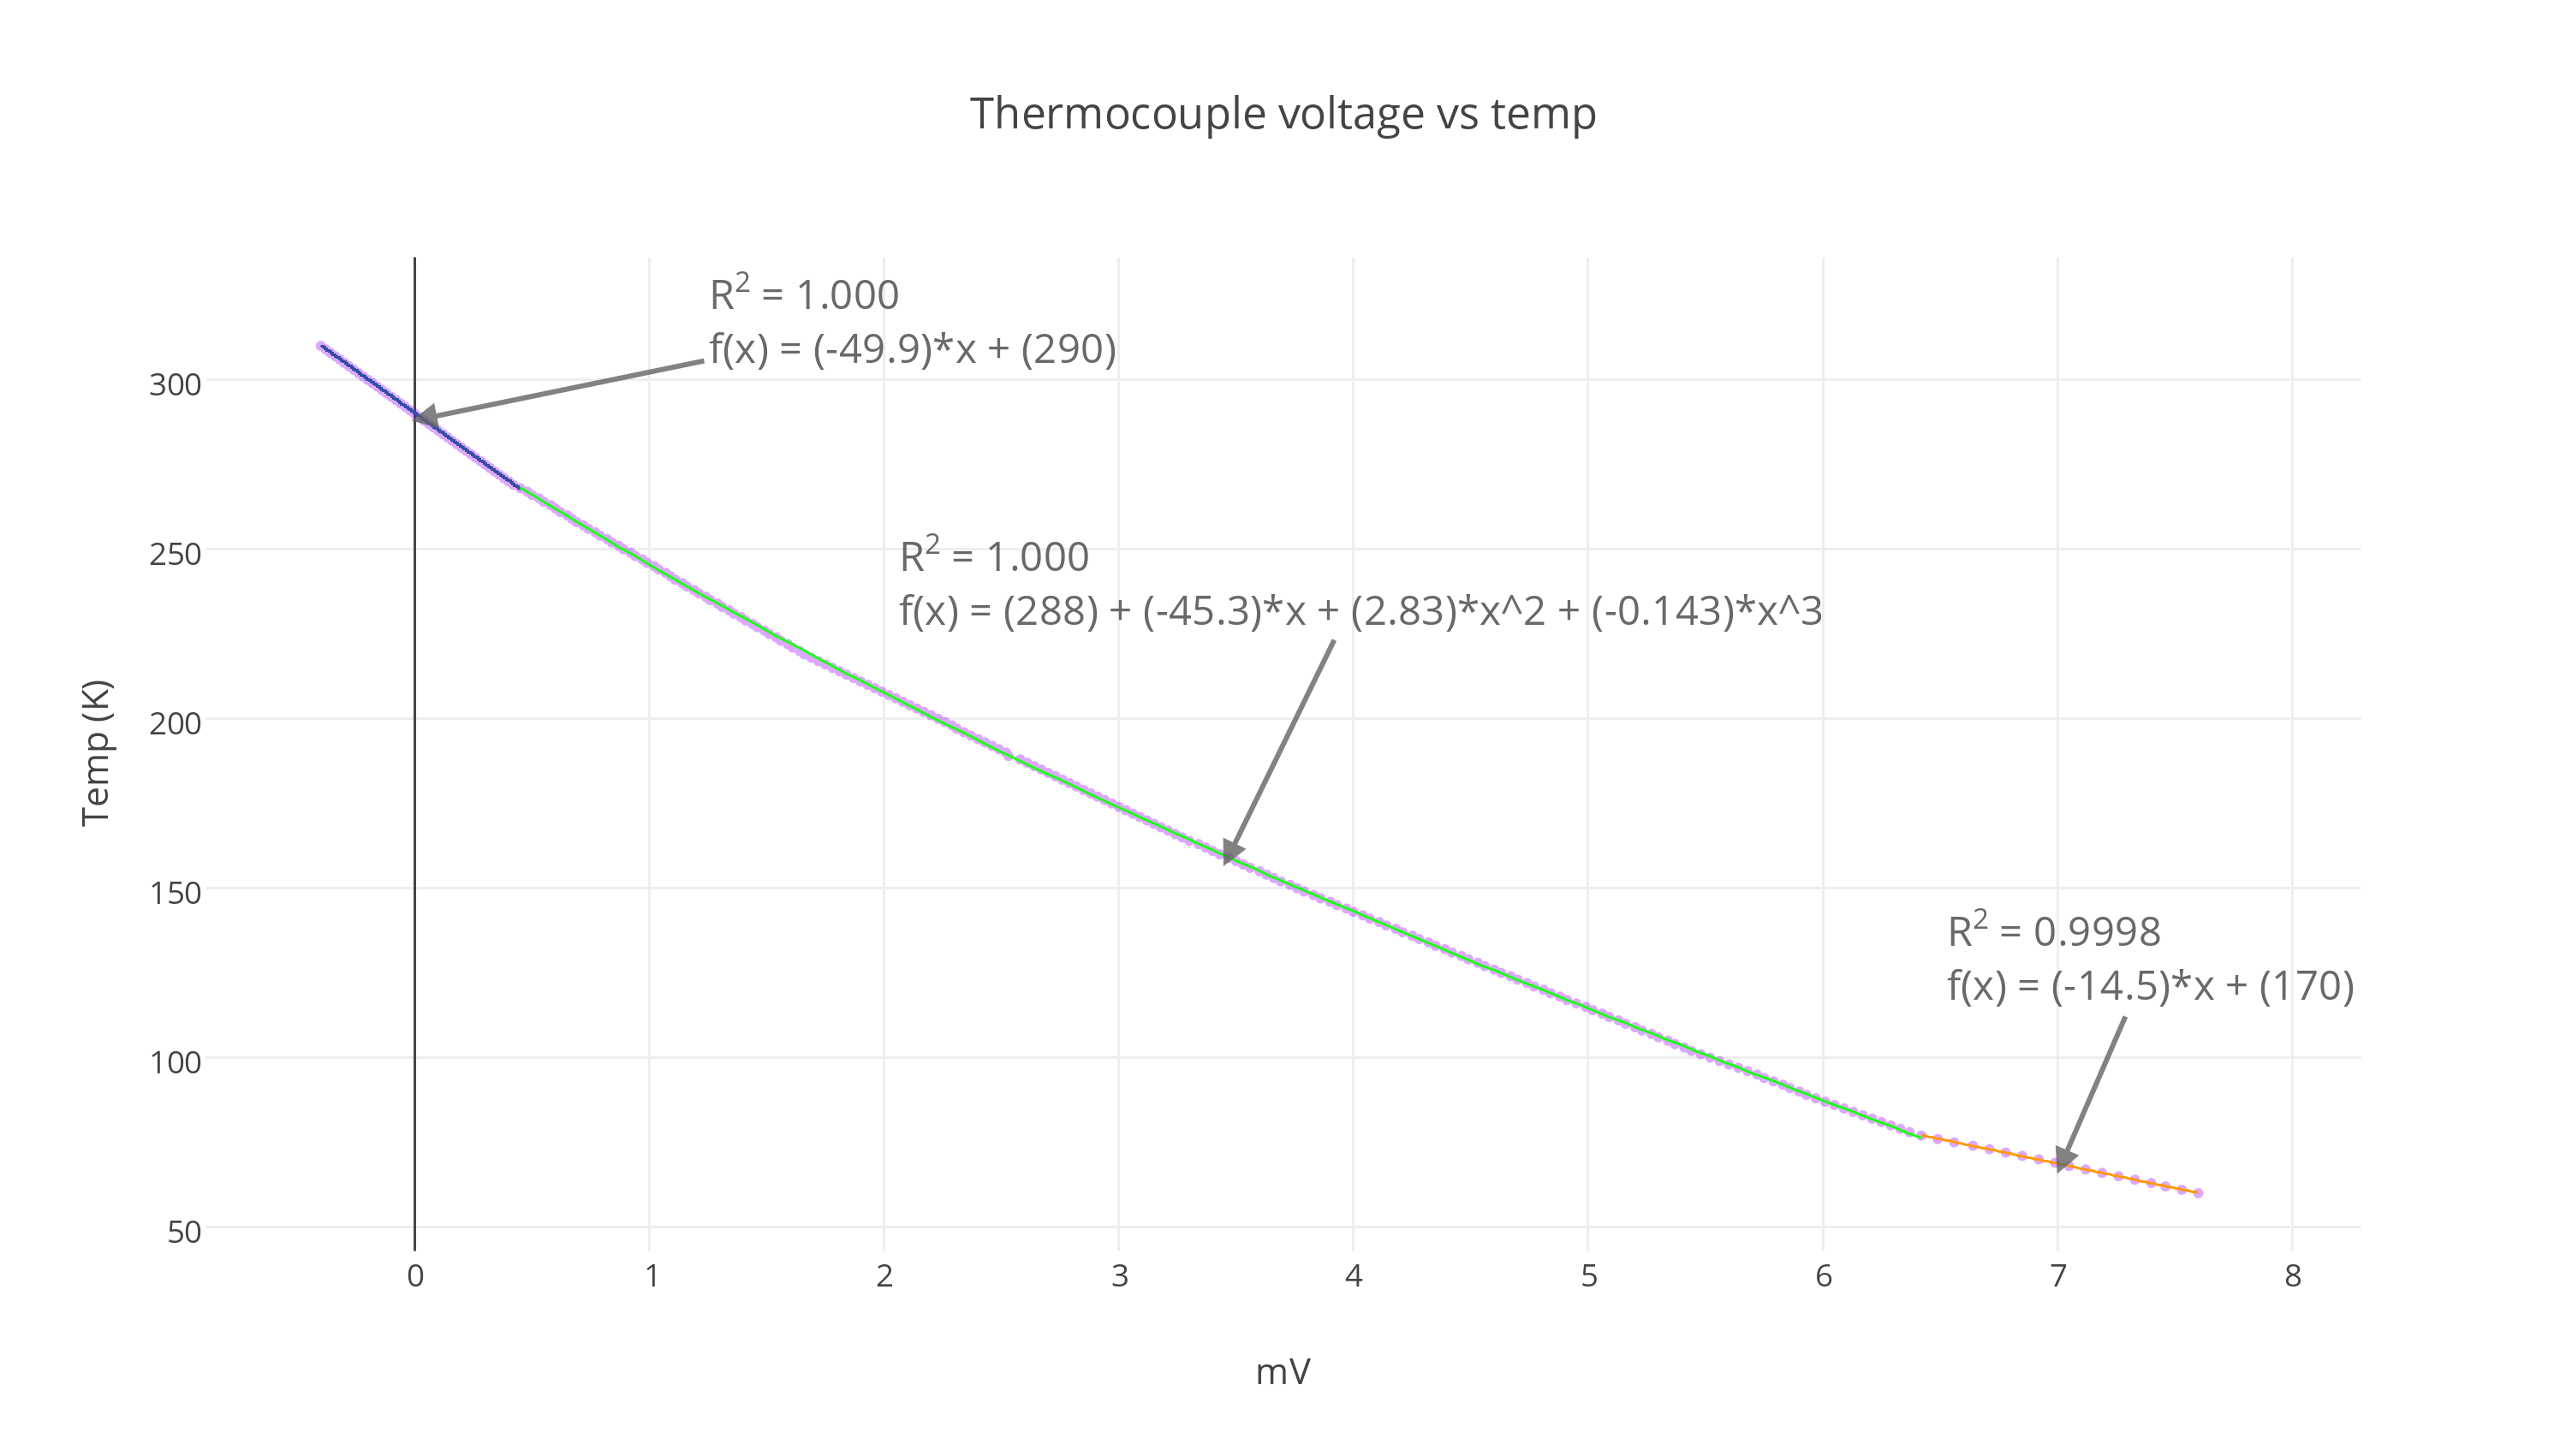
\includegraphics[width=7in]{thermocouple_voltage_vs_temp.png}
\caption{Plot of temperature vs thermocouple voltage transcribed from the Colorado Superconductor Inc experiment manual, with fit lines across different sections.}
\label{TCplot}
\end{figure}

\begin{figure}[h!]
\centering
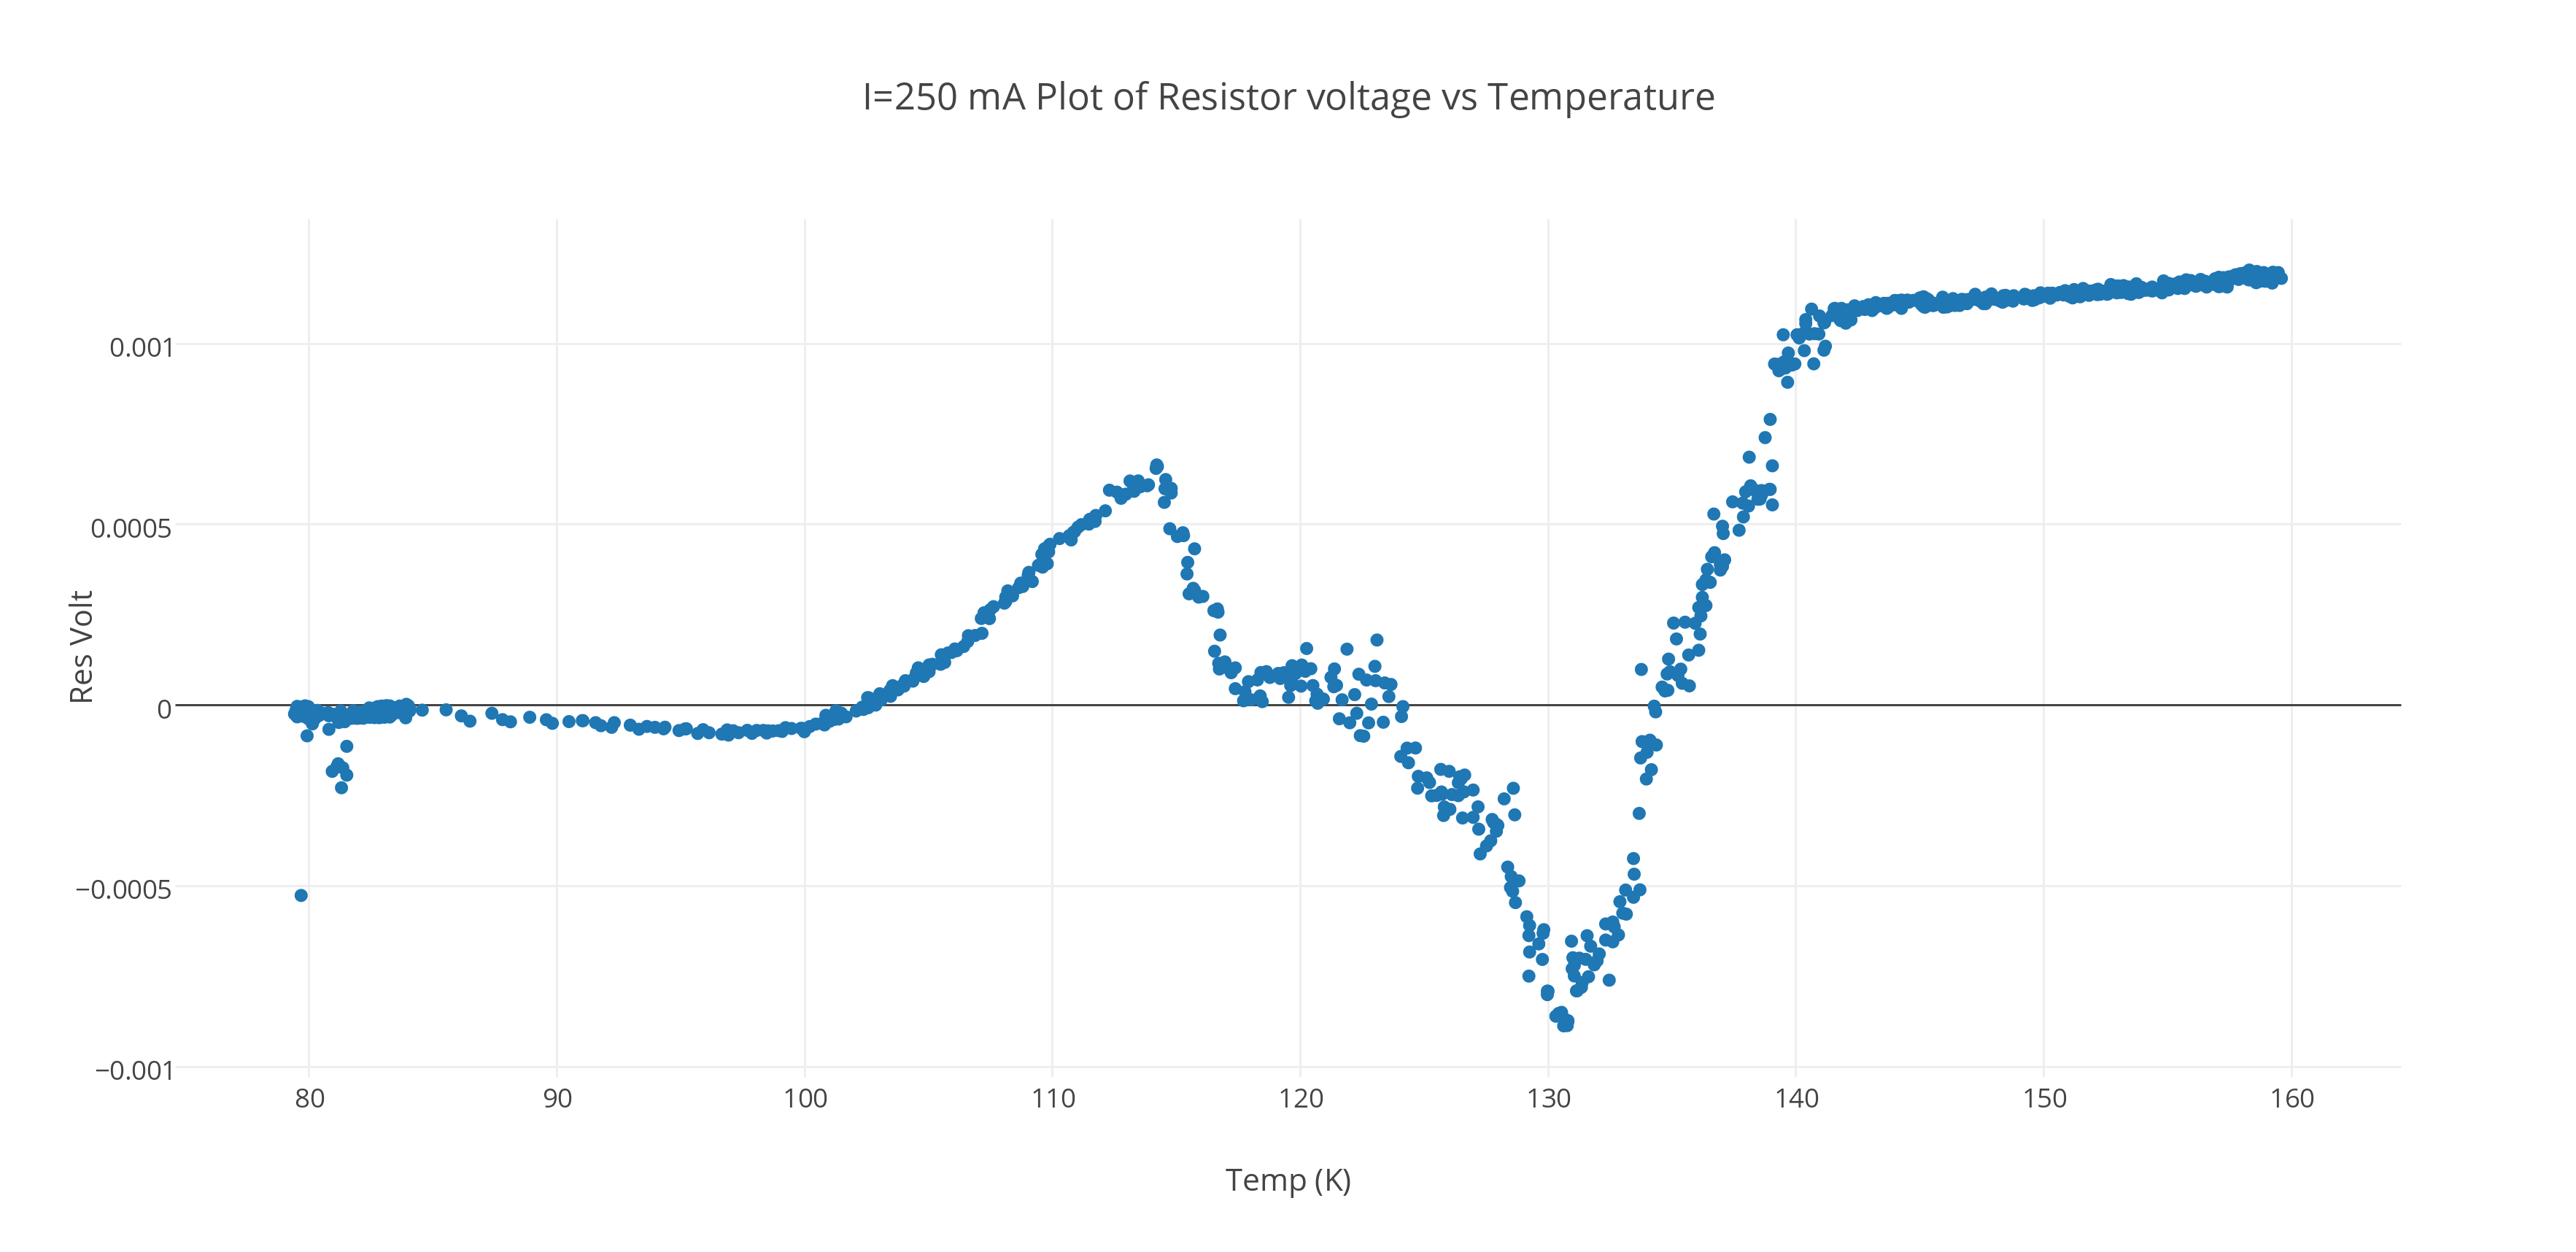
\includegraphics[width=7in]{i250_ma_plot_of_resistor_voltage_vs_temperature.png}
\caption{Plot of resistor voltage vs temperature for a current of 250mA, with rebound effect representative of trials with currents above 1mA.}
\label{ReboundPlot}
\end{figure}

To find a reasonable starting current, we ran warm up trials with currents of 250mA, 100mA, 50mA, and 1mA on the YBCO sample. For all voltages above 1mA, when analyzed the resistor voltage vs temperature graphs displayed a bizarre rebound effect where there would be an increase in resistance before a sudden and severe drop, then followed by an increase into non-superconductivity (see Fig \ref{ReboundPlot}). As a result, we took our main data using 1mA current. We gathered data at 1mA across two warm-ups of the YBCO sample, the first at equal time intervals between points (see Fig. \ref{YBCOplot1}) and the second focusing on taking more points during the transition period than elsewhere (see Fig. \ref{YBCOplot2}).

In order to determine the critical temperature, we located the point along the transition period curve that was halfway between the trend line for resistance during non-superconductivity and the trend line for resistance during superconductivity, and noted the corresponding temperature. The error in our voltage readings was very low (on the order of 0.000005mV). The larger error contribution is related to the width of the transition zone. Defining the positive error as the temperature point where the resistance is at 90\% of the non-superconducting edge, and the negative error as the temperature point where the resistance is at 10\% of the non-superconducting edge, we obtained a range of  91K to 100K and 94K to 101K, for each trial respectively. This yields a final result of $T_{C}=98.03\textrm{K}\pm7\textrm{K}$ and $T_{C}=98.67\textrm{K}\pm4.67\textrm{K}$, respectively (using the greater of the positive and negative error to be conservative).
 
\begin{figure}[h!]
\centering
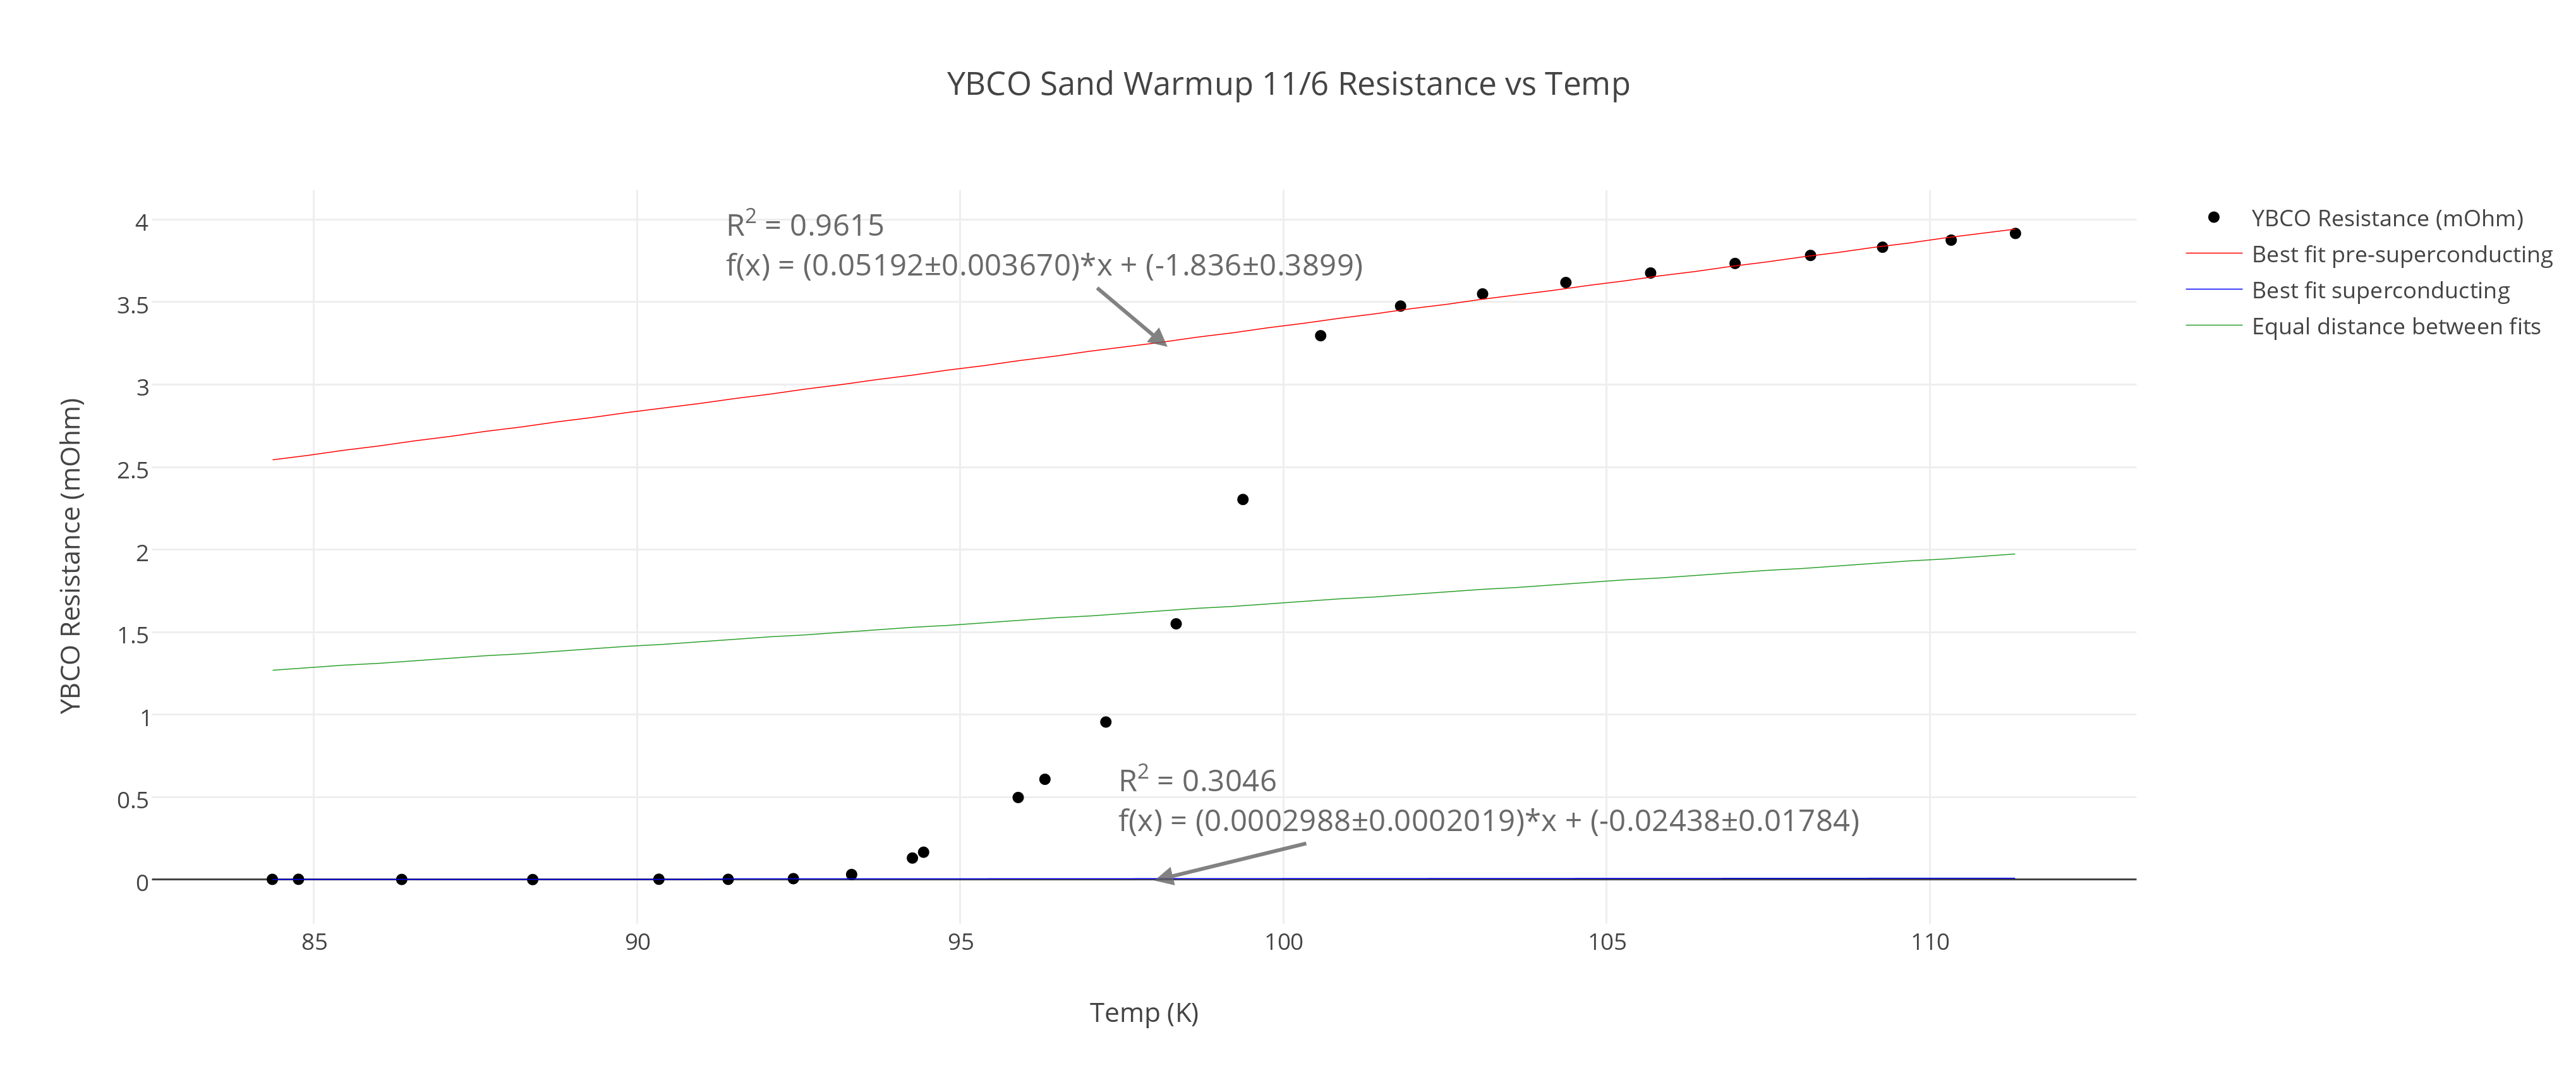
\includegraphics[width=7in]{ybco_sand_warmup_116_resistance_vs_temp.png}
\caption{Plot of resistance vs temperature for YBCO sample, with best fit lines during normal conductivity and during superconductivity, with a third line showing the space equidistant between. Data was gathered every 20 seconds during warm-up.}
\label{YBCOplot1}
\end{figure}

\begin{figure}[h!]
\centering
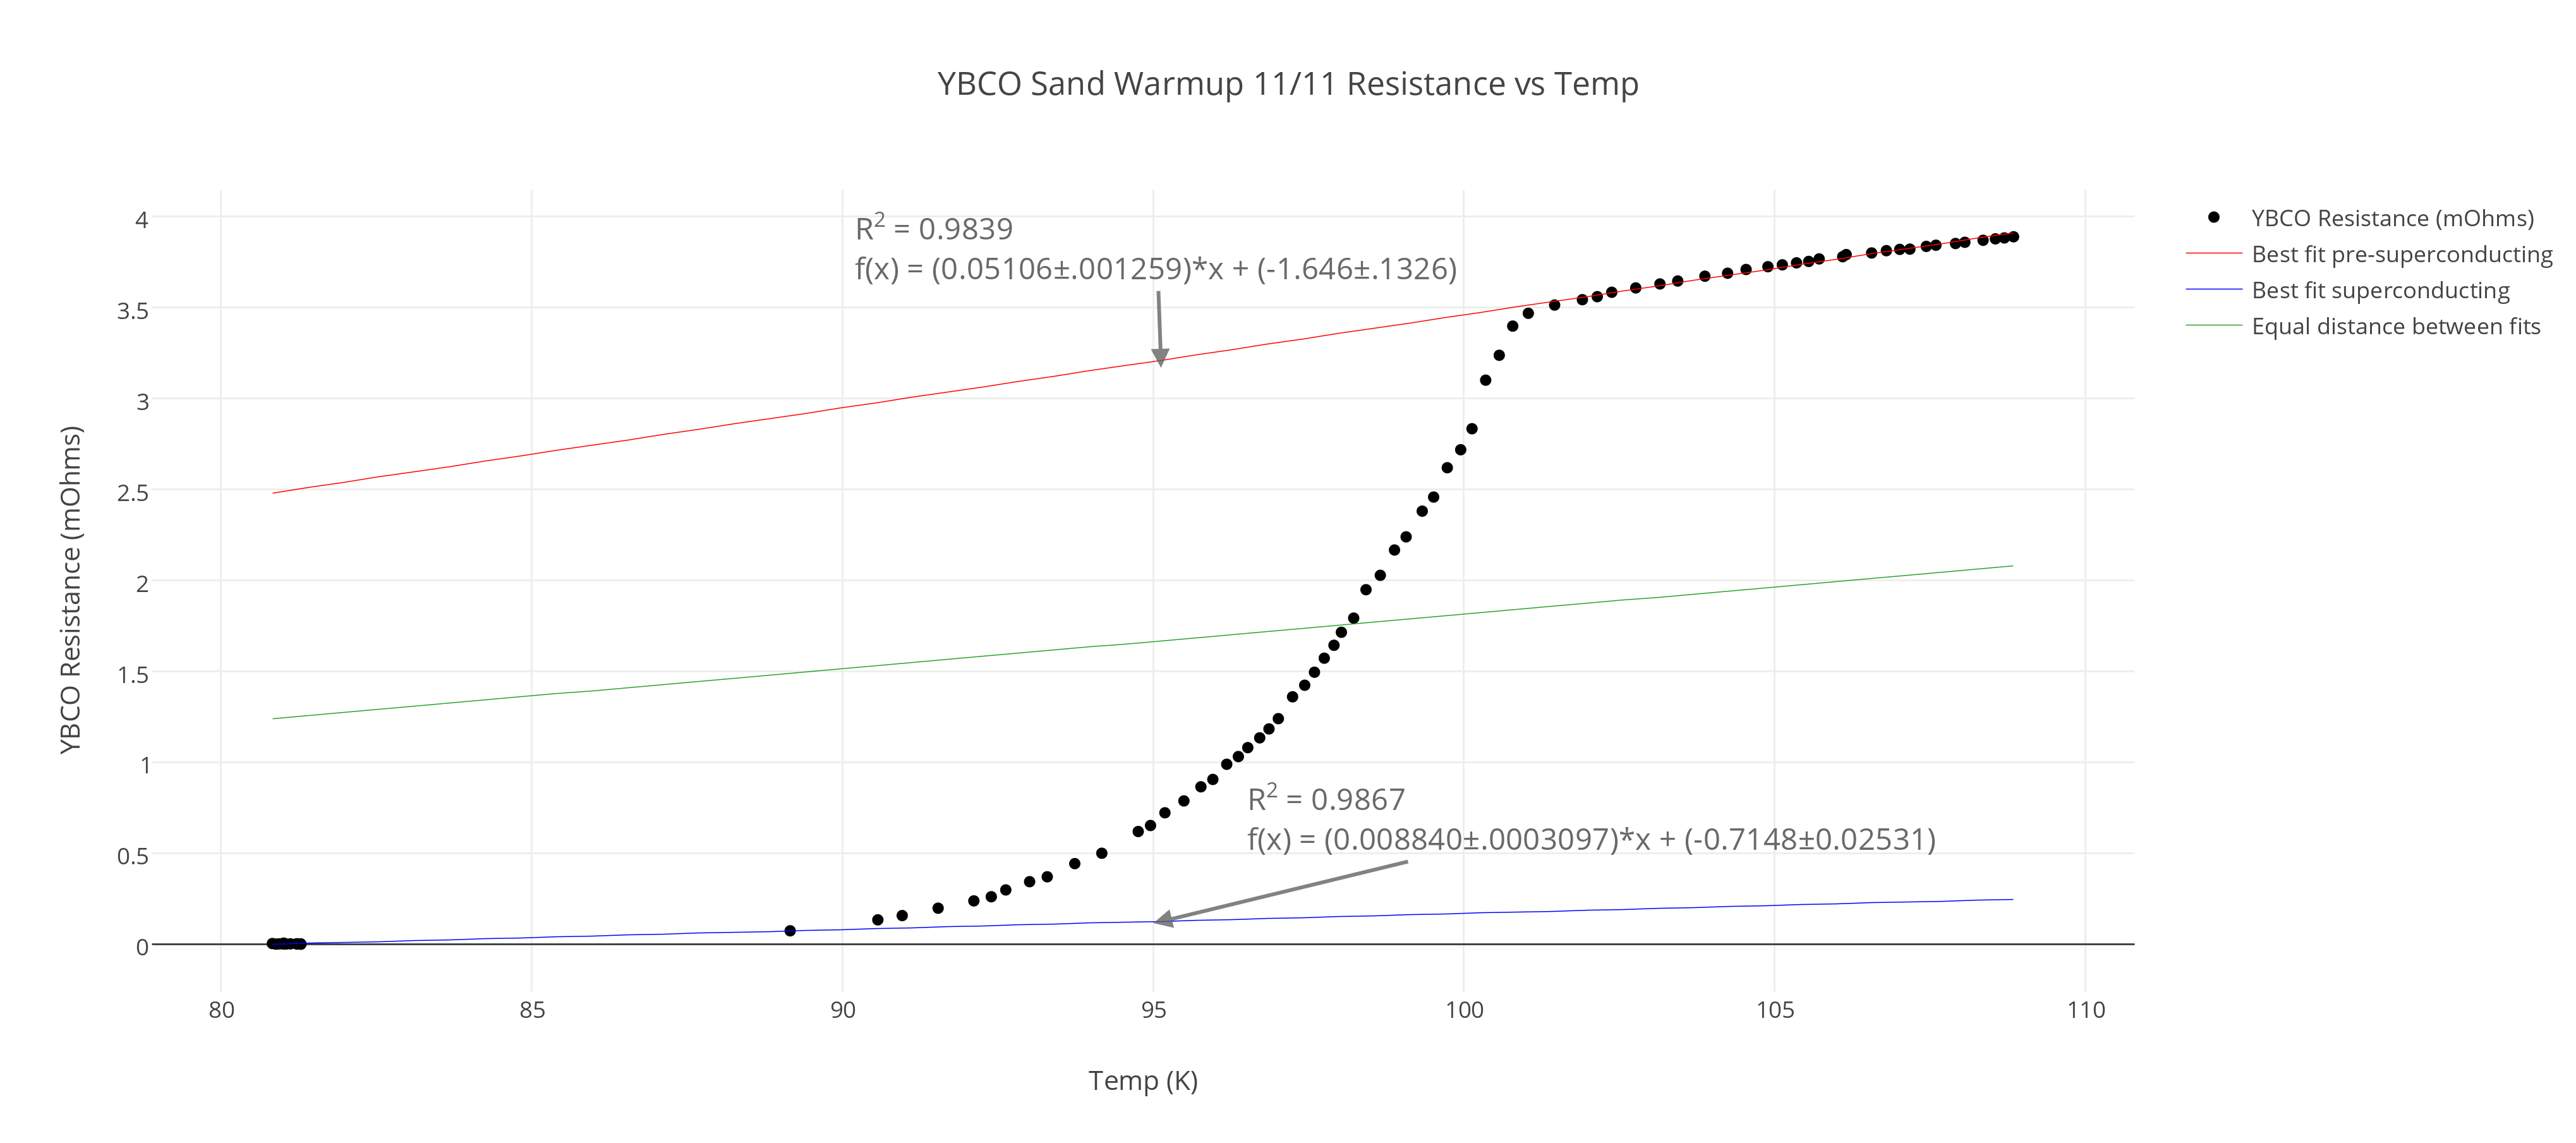
\includegraphics[width=7in]{ybco_sand_warmup_1111_resistance_vs_temp.png}
\caption{Plot of resistance vs temperature for YBCO sample, with best fit lines during normal conductivity and during superconductivity, with a third line showing the space equidistant between. Data was gathered every 30 seconds until onset of superconductivity, then every couple seconds throughout the transition period.}
\label{YBCOplot2}
\end{figure}

\begin{figure}[h!]
\centering
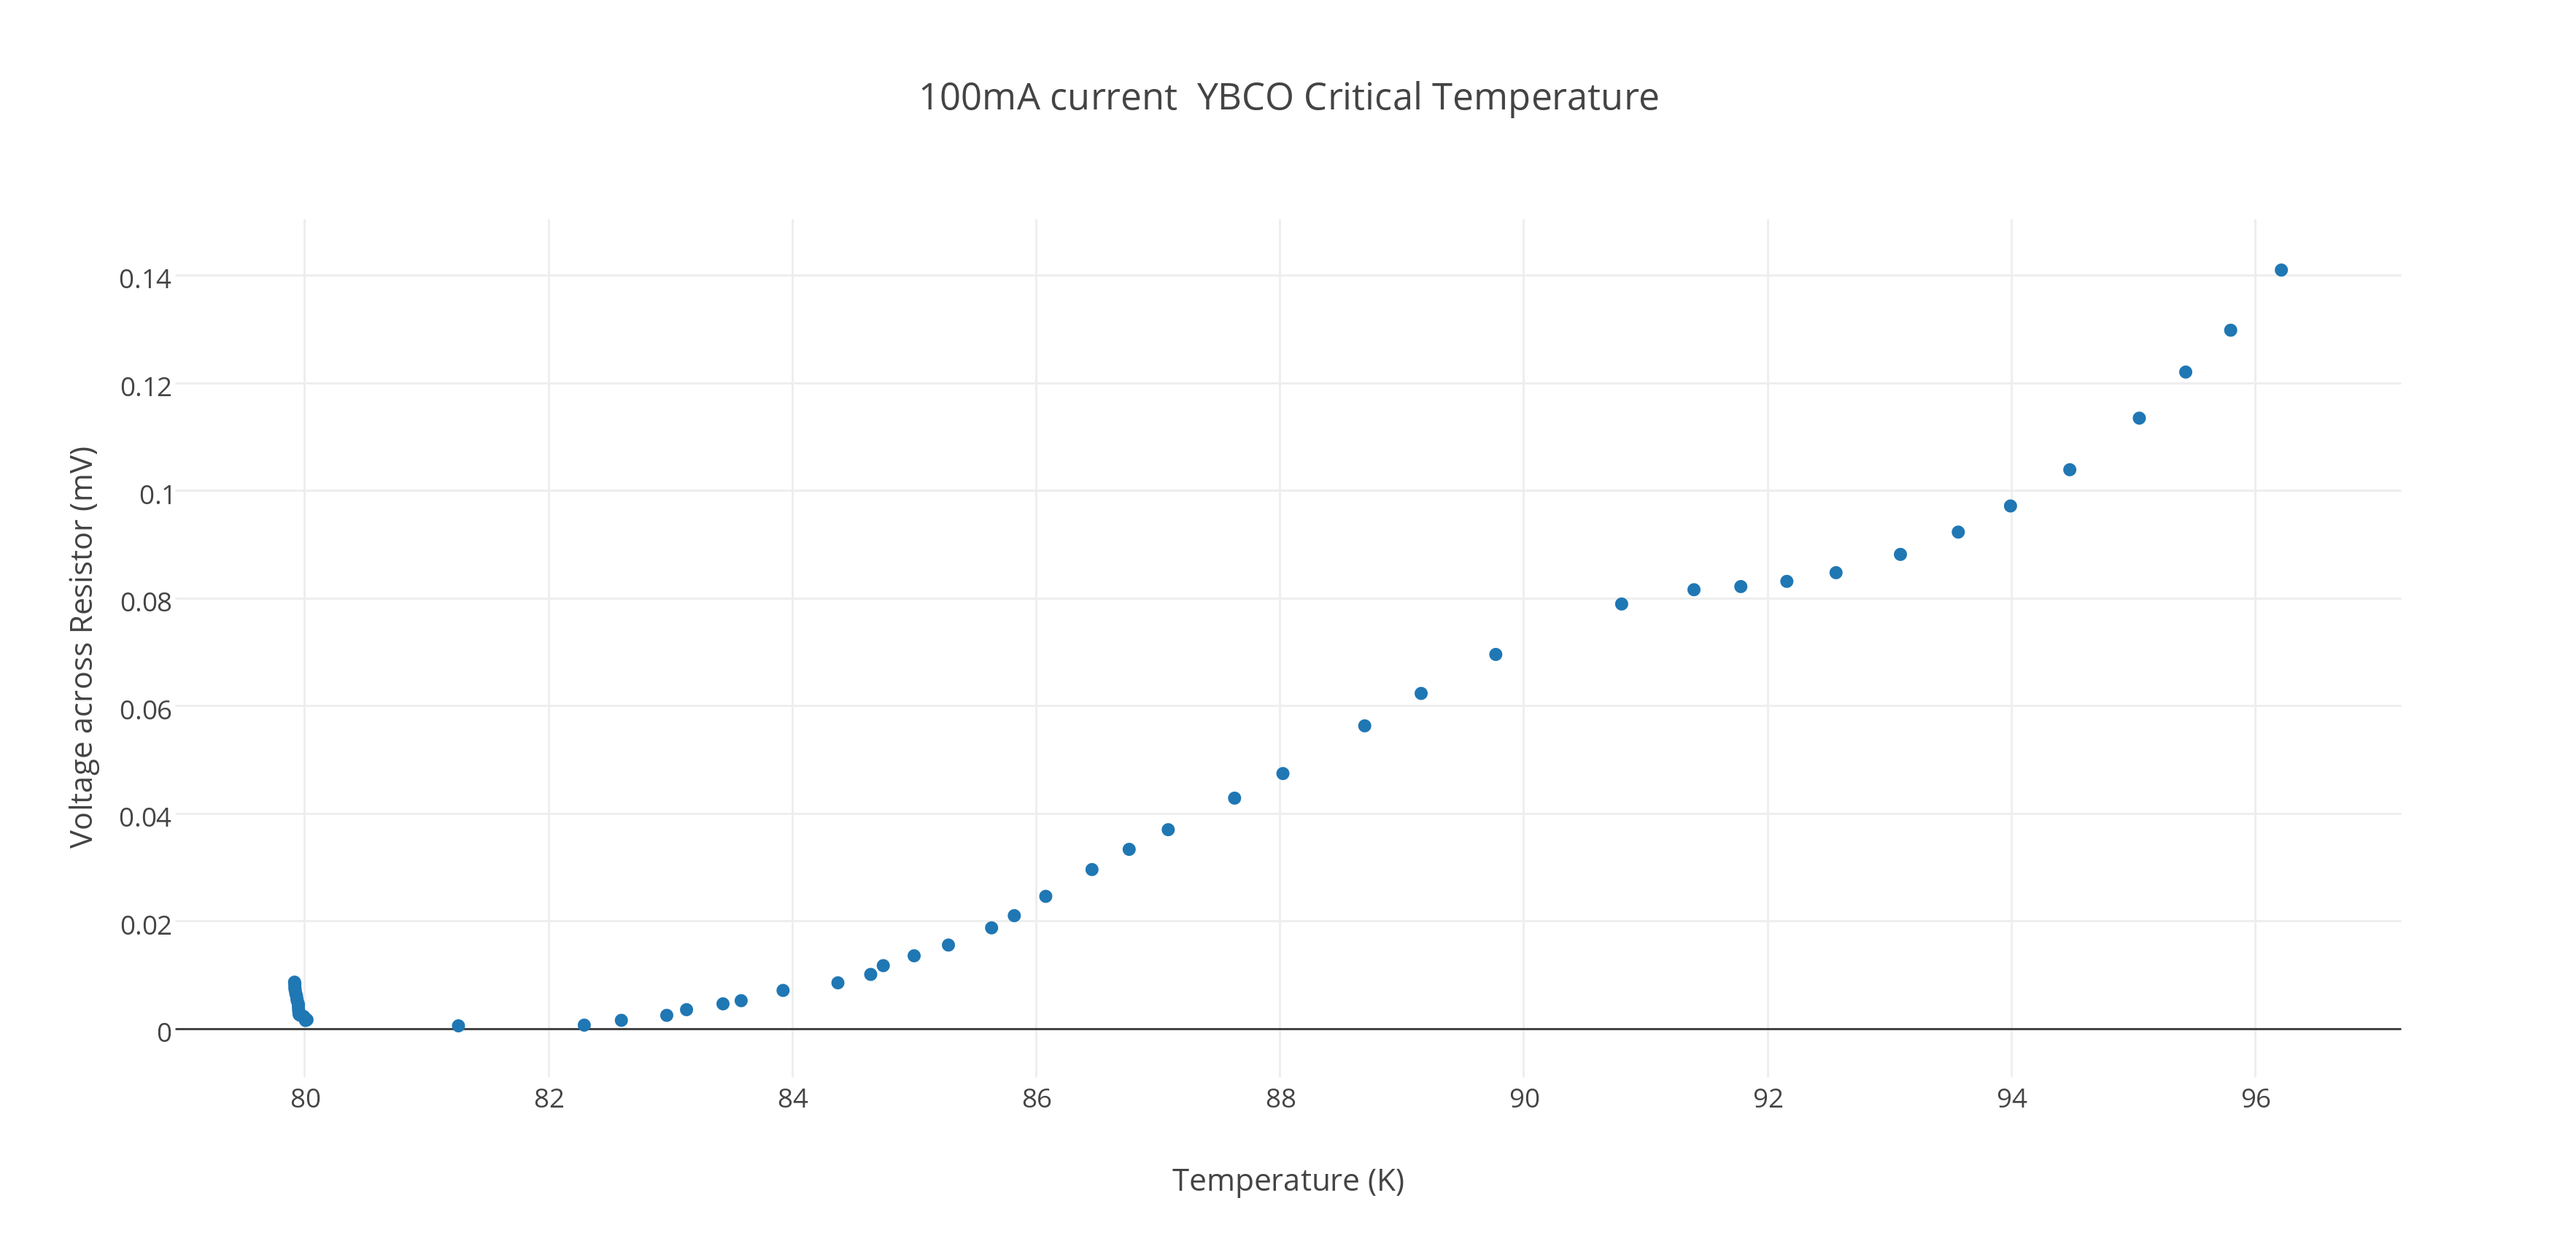
\includegraphics[width=7in]{100ma_current_ybco_critical_temperature}
\caption{Plot of resistor voltage vs temperature for a current of 100mA during transition from superconducting to non-superconducting.}
\label{100mA}
\end{figure}

Despite troubles with rebound at higher currents, a video of the transition from superconducting to non-superconducting at a current of 100mA was obtained, and is shown in Fig \ref{100mA}. While the shaped following the rebound is distorted, and it is hard to identify a single point as the critical temperature – given the double curve effect – the 1mA YBCO trial is superconducting above 90K while the 100mA the sample has already begun the transition and has left pure superconducting by 90K.

Next we looked at a sample of BSCCO gathered through the two-phase lock-in amplifier. Only one trial was performed, though data was gathered every 3 seconds for 3 hours. Once the data was plotted, the same procedure was used as with the YBCO sample to determine the critical temperature (see Fig. \ref{BSCCOplot1}). The critical temperature $T_C$ here was 110K, with a range of 101K to 119K (10\% to 90\%) for an error of $\pm$ 9K. Of particular interest was the trend during the early pre-superconducting period. While certainly not truly ceasing to superconduct, there appeared to be some jumps in resistance during the superconductive phase, shown closely in Fig. \ref{BSCCOplot2}. On closer inspection, while there is clearly some upward trend and movement not seen in the YBCO sample, it is not clear enough to pinpoint any specific jumps.

\begin{figure}[h!]
\centering
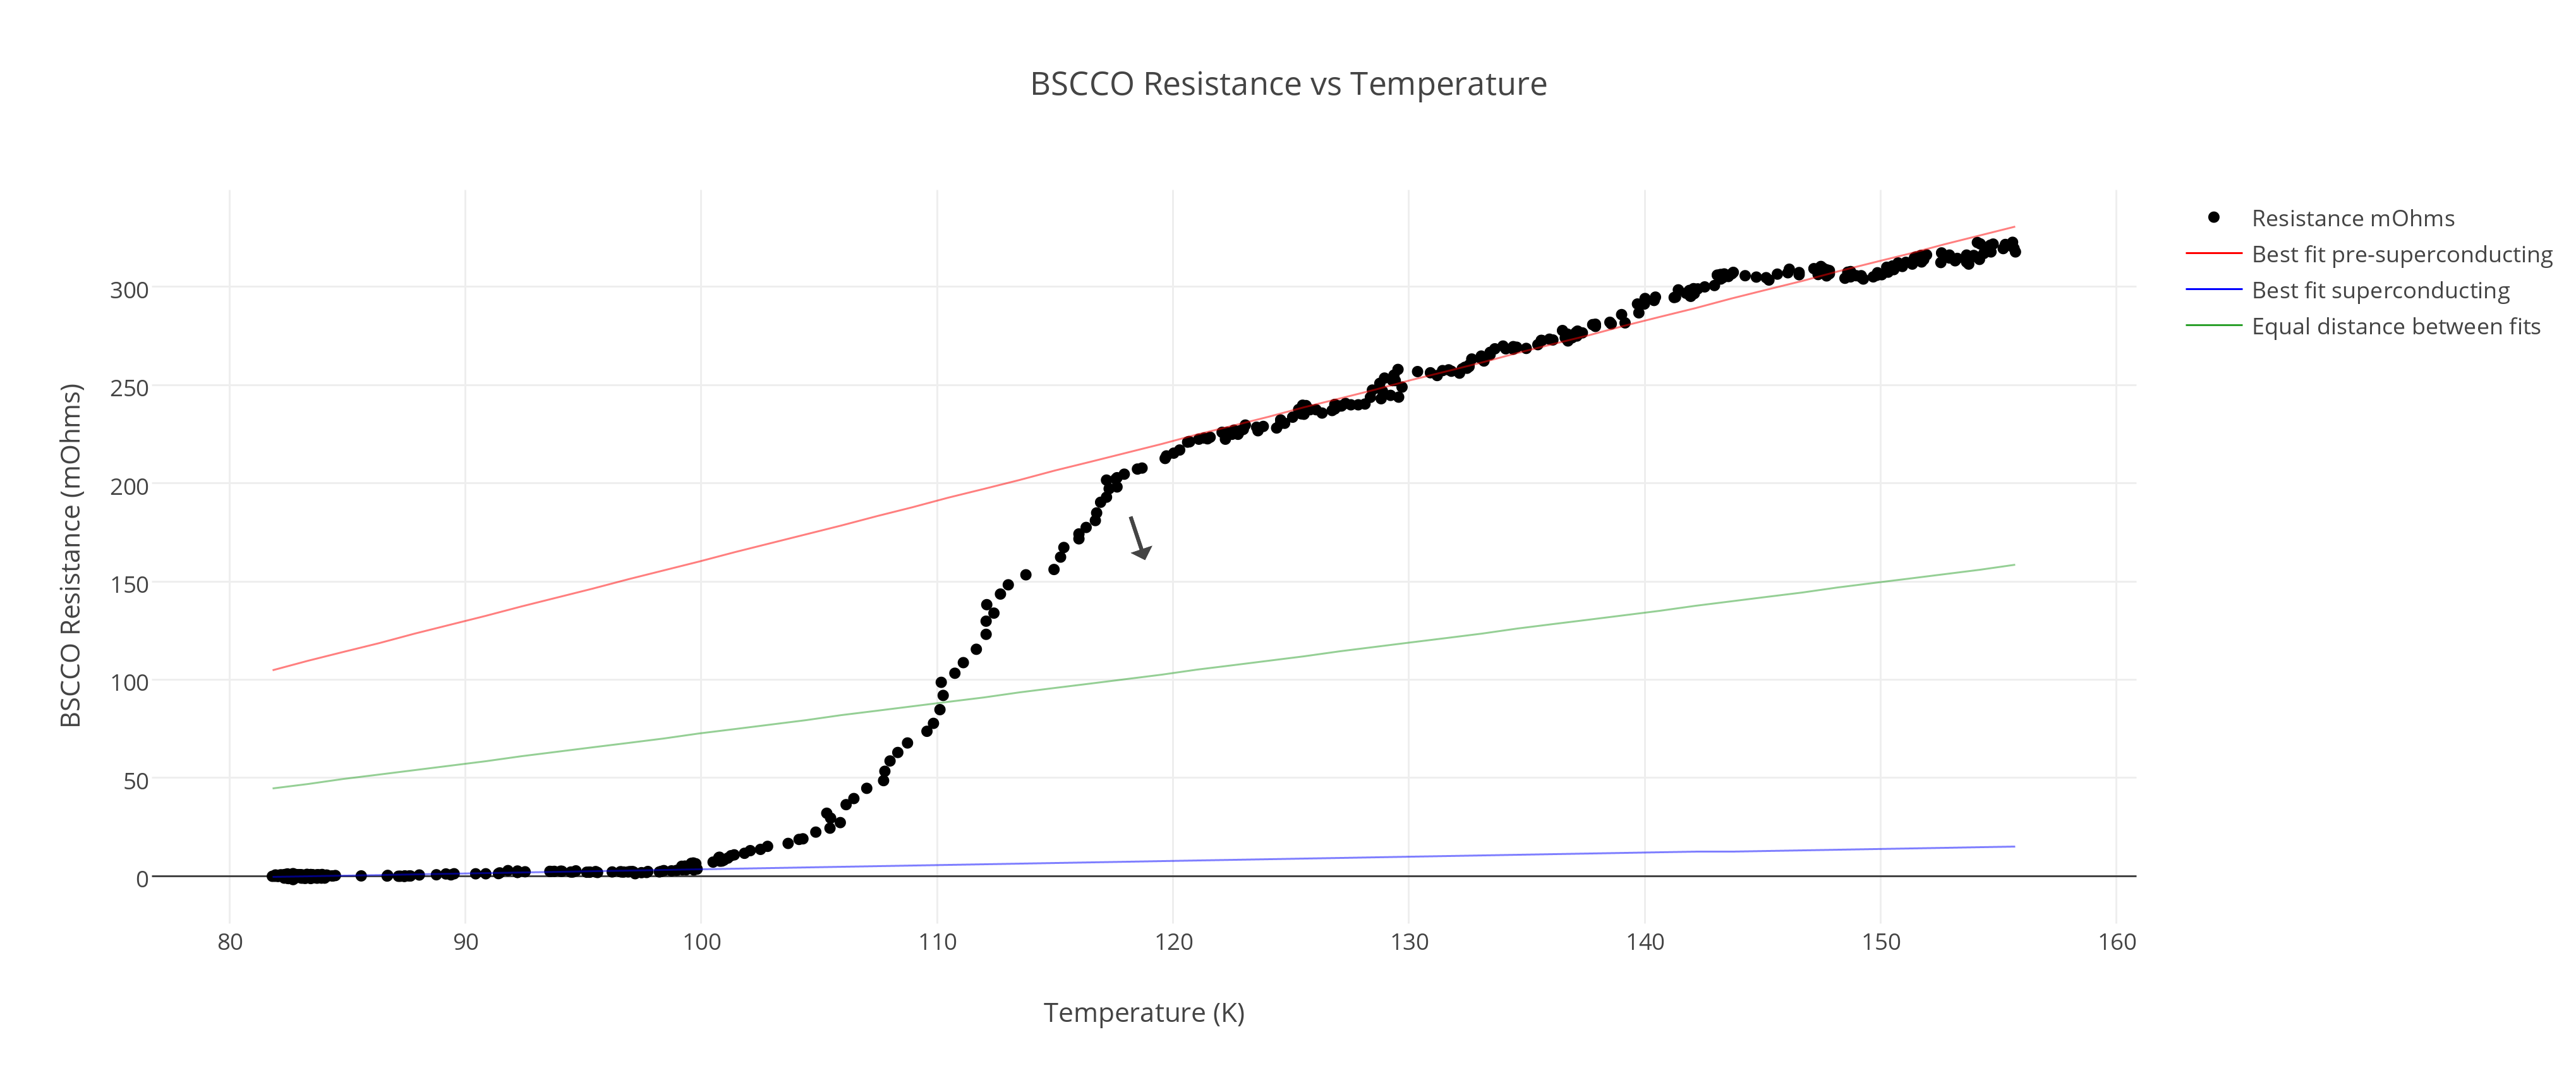
\includegraphics[width=7in]{bscco_resistance_vs_temperature.png}
\caption{Plot of resistance vs temperature for BSCCO sample, with best fit lines during normal conductivity and during superconductivity, with a third line showing the space equidistant between.}
\label{BSCCOplot1}
\end{figure}

\begin{figure}[h!]
\centering
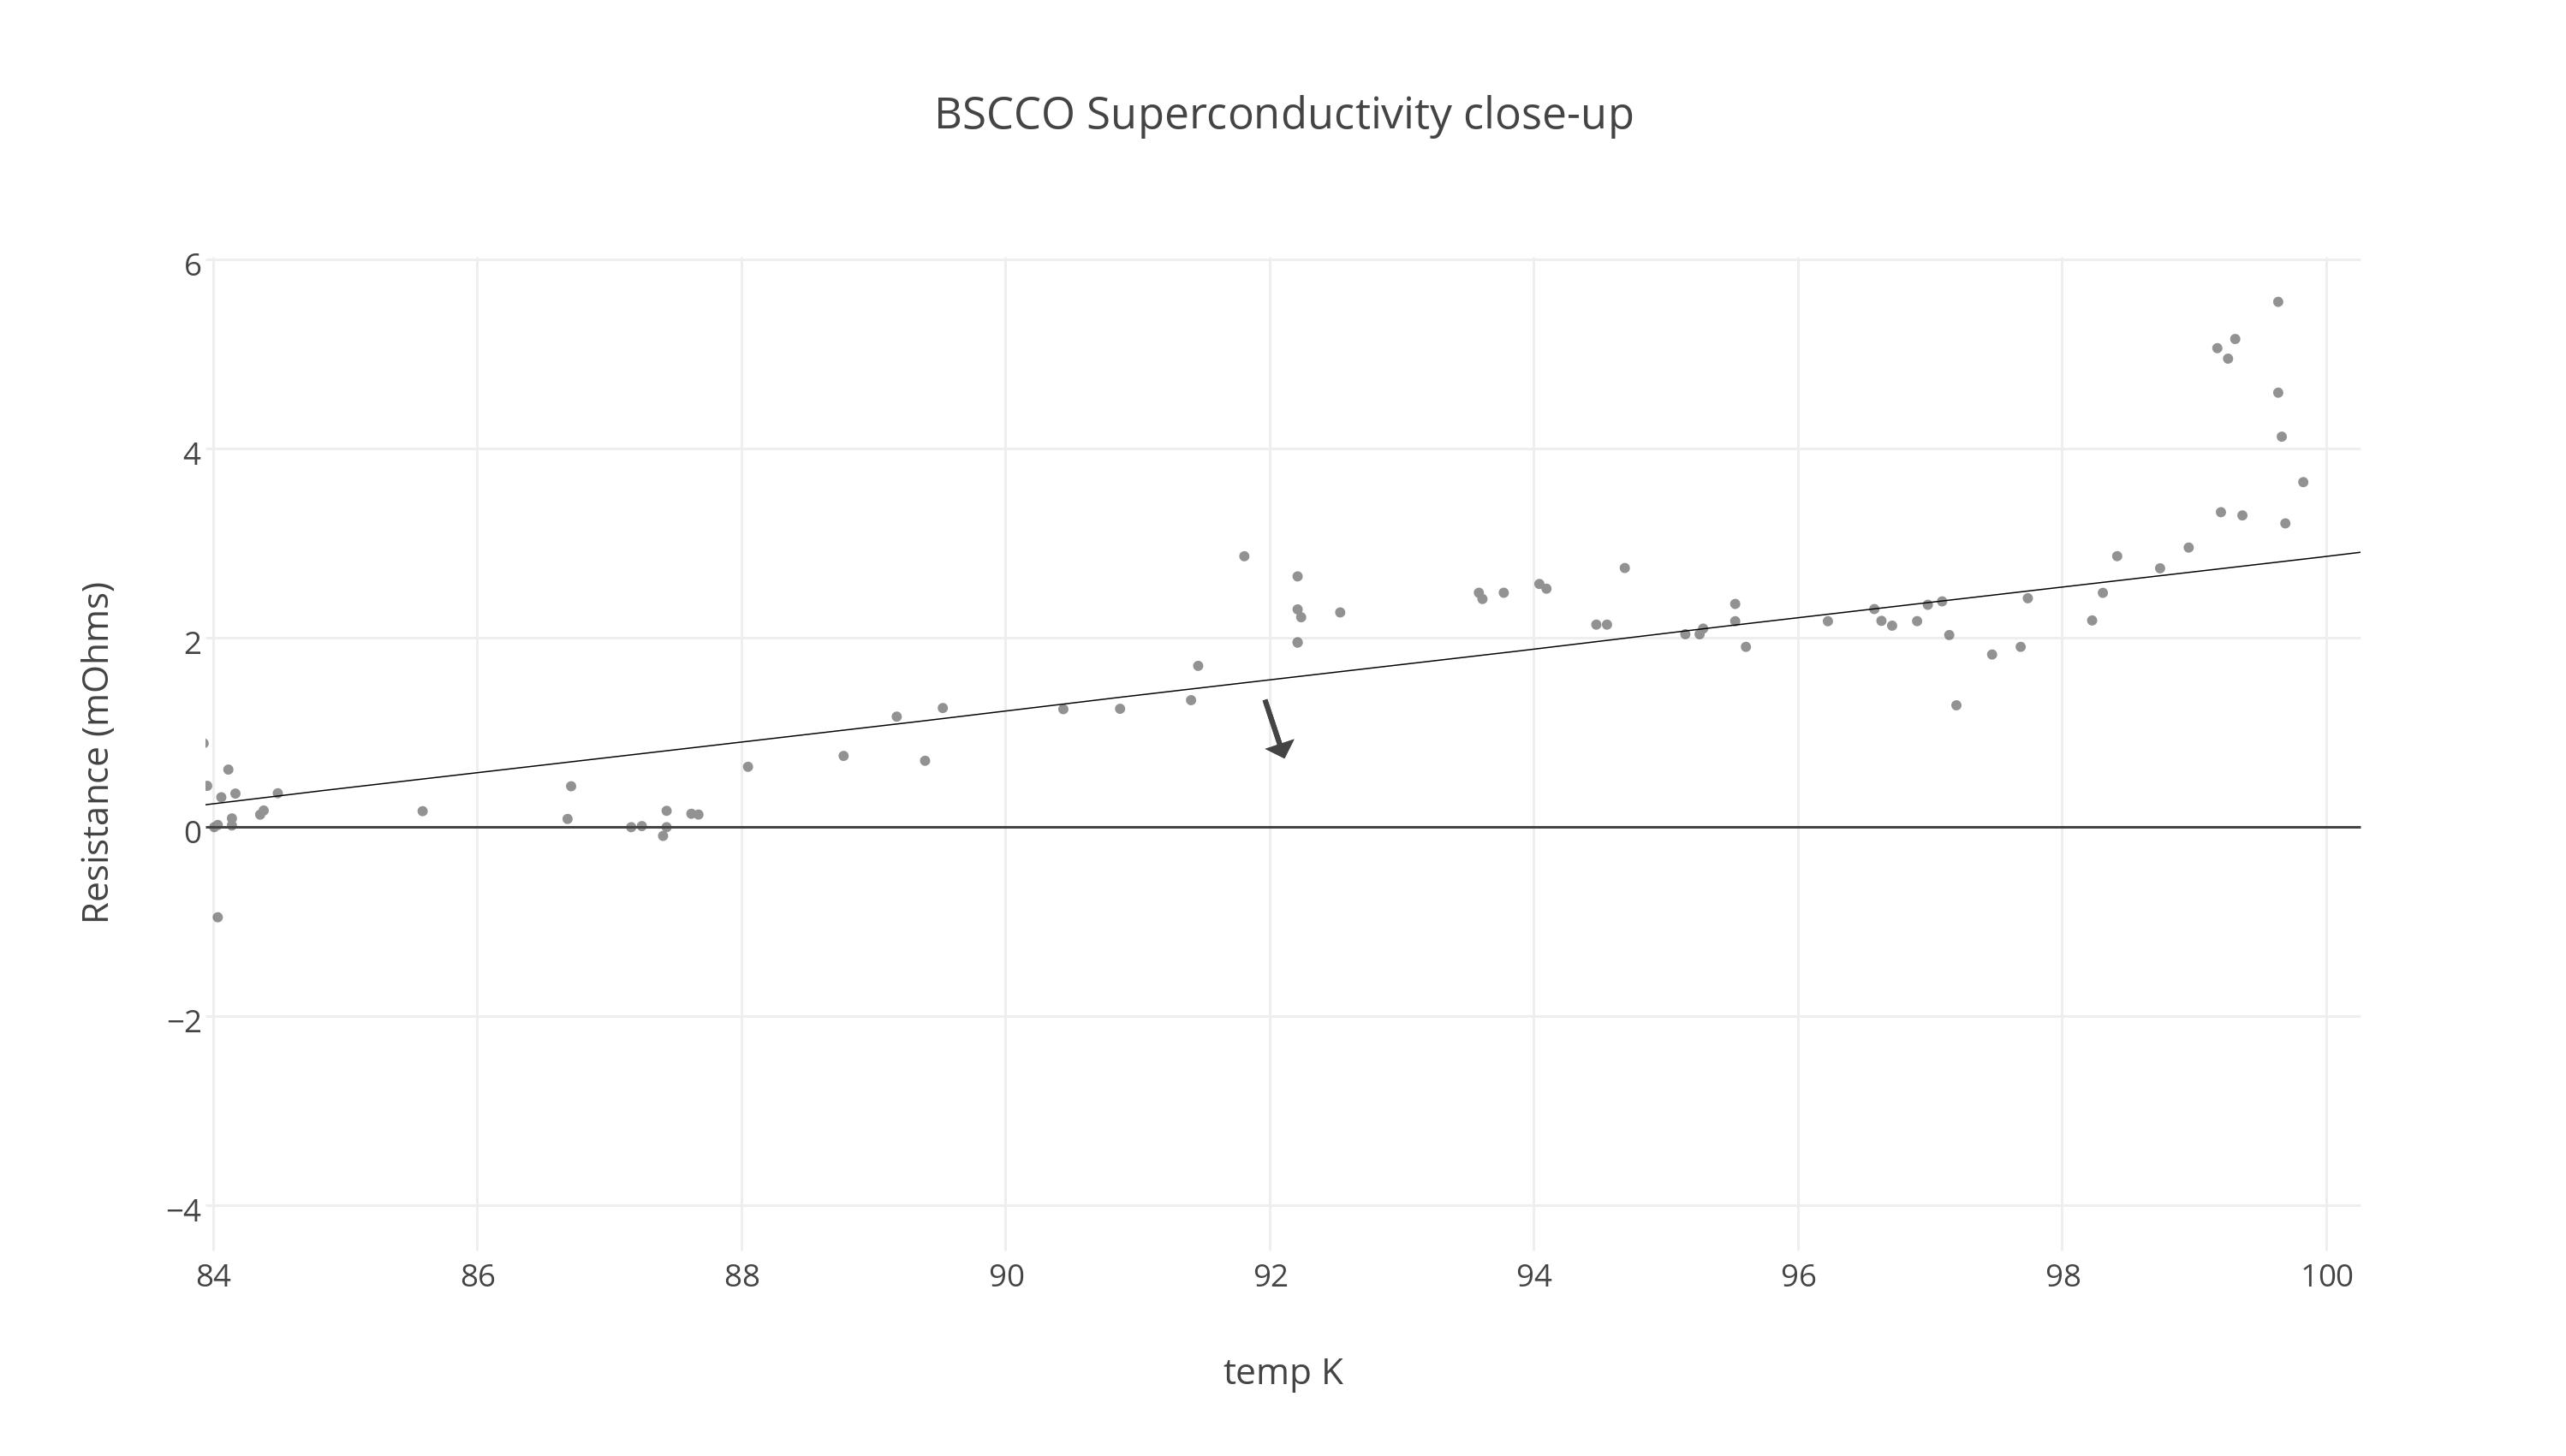
\includegraphics[width=7in]{bscco_superconductivity_close-up.png}
\caption{Close up of the BSCCO sample warm-up during it superconductive phase. Irregularities are definitely present, but jumps are not clear.}
\label{BSCCOplot2}
\end{figure}

\section{Conclusion}

Superconductivity was clearly achieved in both the YBCO and the BSCCO samples, and their transition to being non-superconductive as their temperature increased was recorded. Graphical analysis yielded a critical temperature for YBCO of 98.35K $\pm$ 7K (averaged between the two trials) and for BSCCO of 110K $pm$ 9K. According to the Colorado Superconductor Inc manual, YBCO has a critical temperature of 92K, which is within our margin of error; similarly, the BSCCO sample was noted as having a critical temperature of 105K, again within our margin of error. The strange behavior seen during the end of the superconducting phase of the BSCCO sample may also have had to do with the fact that BSCCO can have two other critical temperatures. The general formula is $\text{Bi}_{2,1}\text{Sr}_{n+1}\text{Ca}_{\text{n}-1}\text{Cu}_{\text{n}}\text{O}_{2n+4+\delta}$. While the sample we had was specified for $n=3$, it is quite possible that other variations were present in our sample, each with their own critical temperature: $T_C$ for $n=1$ is 80K and $T_C$ for $n=2$ is 90K. \cite{colo} While we did not get as cold as 80K, we could be seeing some sections stop superconducting around 90K, alongside the already non-superconducting $n=1$ material, giving us a not truly flat superconducting zone. Finally, looking at the transition for YBCO with a current of 100mA, despite problems identifying a strict number for the critical temperature, the transition to non-superconducting clearly happens at a lower temperature then for 1mA. This is consistent with expectations since more energy from the increased current means that less thermal energy from warming up is needed to impart enough energy to stop the superconducting state within the YBCO crystals.


\begin{thebibliography}{99}
% The numeral (here 99) in curly braces is nominally the number of entries in
% the bibliography. It's supposed to affect the amount of space around the
% numerical labels, so only the number of digits should matter--and even that
% seems to make no discernible difference.

\bibitem{intro} Charles Poole, Horacio Farach, and Richard Creswick, \textit{Superconductivity} (Academic Press, 2007).

\bibitem{kumar} Ajay Kumar Saxena, \textit{High-Temperature Superconductors} (Springer Berlin Heidelberg, 2010).

\bibitem{colo} Experiment Guide for Superconductor Demonstrations. Colorado Superconductor Inc., Version 7.0, May 2007.

\bibitem{ybcotemp} R. J. Cava, B. Batlogg, R. B. van Dover, D. W. Murphy, S. Sunshine, T. Siegrist, J. P. Remeika, E. A. Rietman, S. Zahurak, and G. P. Espinosa, "Bulk superconductivity at 91 K in sngle-phase oxygen-deficient perovskite $\text{Ba}_2\text{YCU}_3\text{O}_{9-\delta}$, Phys. Rev. Letters 58, 1676 (1987).

\bibitem{temps} J. M. Tarascon, W. R. McKinnon, P. Barboux, D. M. Hwang, B. G. Bagley, L. H. Greene, G. W. Hull, Y. LePage, N. Stoffel, and M. Giroud, "Preparation, structure, and properties of the superconducting compound series $\text{Bi}_2\text{Sr}_2\text{Ca}_{n-1}\text{Cu}_{n}\text{O}_y$ with $n=1,2,\text{ and }3$", Phys. Rev. B 38, 8885 (1998).

\bibitem{melissinos} Experiments in Modern Physics.  Adrian Constantin Melissinos and Jim Napolitano.  Gulf Professional Publishing, 2003



\end{thebibliography}

% If your manuscript is conditionally accepted, the editors will ask you to
% submit your editable LaTeX source file.  Before doing so, you should move
% all tables and figure captions to the end, as shown below.  Tables come 
% first, followed by figure captions (with figure inclusions commented-out).
% Figures should be submitted as separate files, collected with the
% LaTeX file into a single .zip archive.

%\newpage   % Start a new page for tables

%\begin{table}[h!]
%\centering
%\caption{Elementary bosons}
%\begin{ruledtabular}
%\begin{tabular}{l c c c c p{5cm}}
%Name & Symbol & Mass (GeV/$c^2$) & Spin & Discovered & Interacts with \\
%\hline
%Photon & $\gamma$ & \ \ 0 & 1 & 1905 & Electrically charged particles \\
%Gluons & $g$ & \ \ 0 & 1 & 1978 & Strongly interacting particles (quarks and gluons) \\
%Weak charged bosons & $W^\pm$ & \ 82 & 1 & 1983 & Quarks, leptons, $W^\pm$, $Z^0$, $\gamma$ \\
%Weak neutral boson & $Z^0$ & \ 91 & 1 & 1983 & Quarks, leptons, $W^\pm$, $Z^0$ \\
%Higgs boson & $H$ & 126 & 0 & 2012 & Massive particles (according to theory) \\
%\end{tabular}
%\end{ruledtabular}
%\label{bosons}
%\end{table}

%\newpage   % Start a new page for figure captions

%\section*{Figure captions}

%\begin{figure}[h!]
%\centering
%\includegraphics{GasBulbData.eps}   % This line stays commented-out
%\caption{Pressure as a function of temperature for a fixed volume of air.  
%The three data sets are for three different amounts of air in the container. 
%For an ideal gas, the pressure would go to zero at $-273^\circ$C.  (Notice
%that this is a vector graphic, so it can be viewed at any scale without
%seeing pixels.)}

%\label{gasbulbdata}
%\end{figure}

%\begin{figure}[h!]
%\centering
%\includegraphics[width=5in]{ThreeSunsets.jpg}   % This line stays commented-out
%\caption{Three overlaid sequences of photos of the setting sun, taken
%near the December solstice (left), September equinox (center), and
%June solstice (right), all from the same location at 41$^\circ$ north
%latitude. The time interval between images in each sequence is approximately
%four minutes.}
%\label{sunsets}
%\end{figure}

\end{document}
